\setcounter{figure}{5}
\begin{figure}[H]
\centering
\par\smallskip\textbf{Panel S6; provisional numerical counterpart: partially reproduced}\par
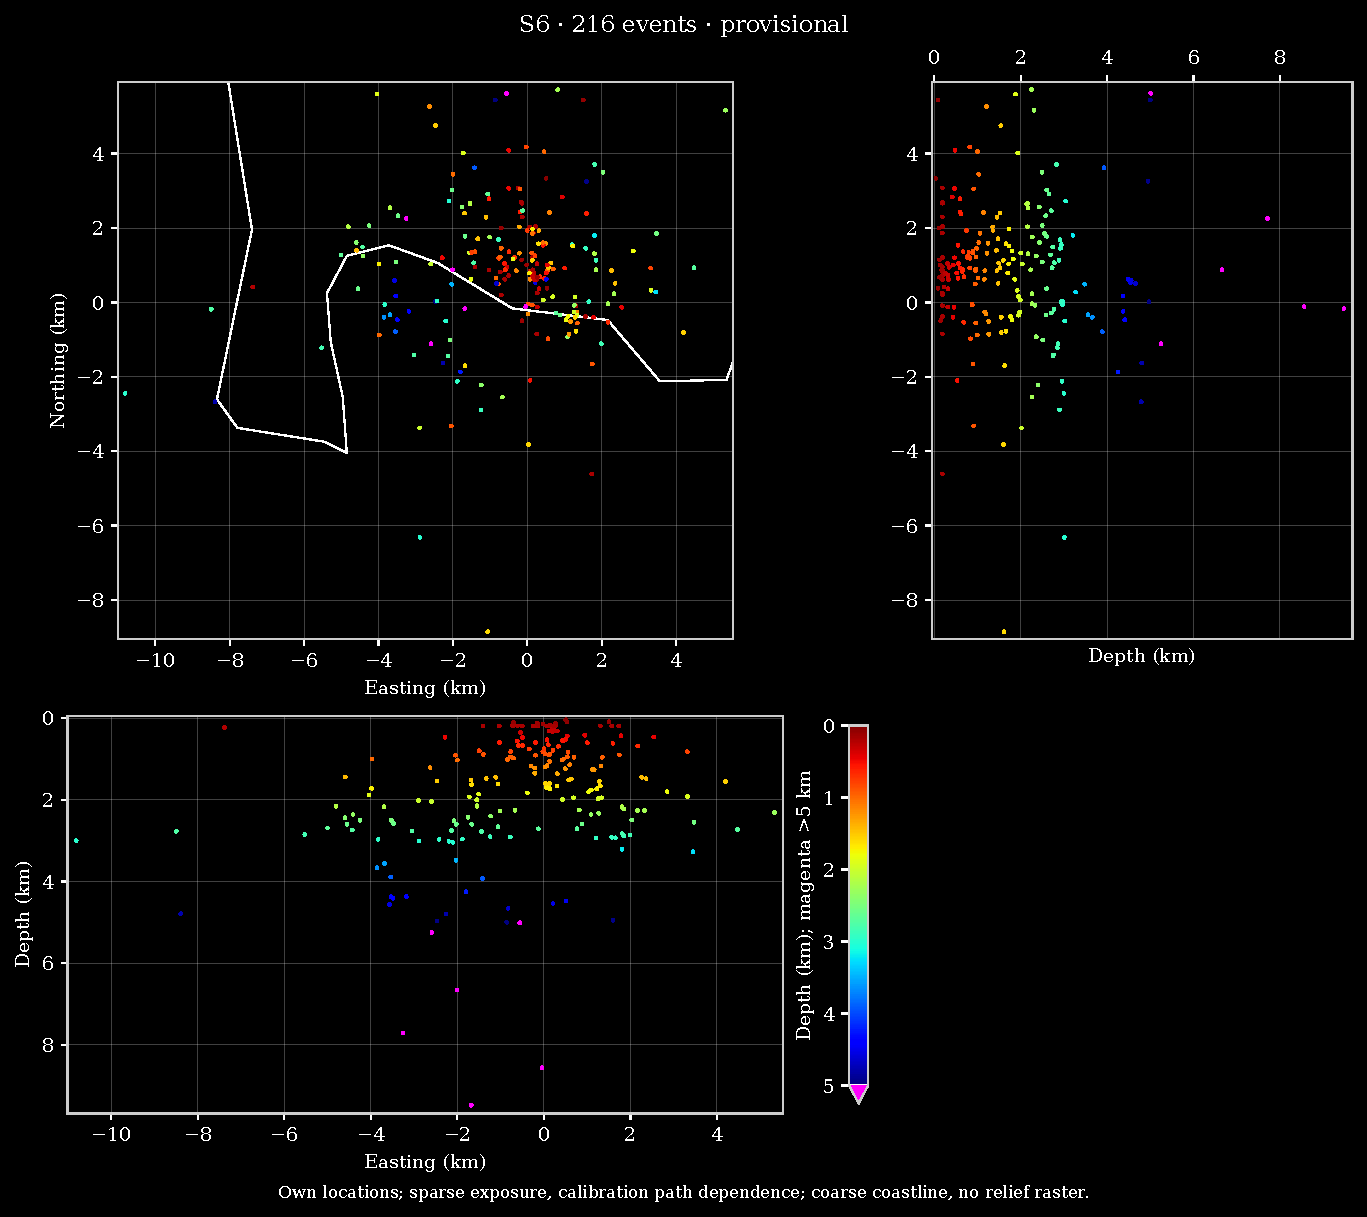
\includegraphics[width=.94\linewidth,height=0.310\textheight,keepaspectratio]{figures/figure_S6_provisional.pdf}
\par\smallskip\textbf{Panel Latest extended cohort: independently rerun, provisional: partially reproduced}\par
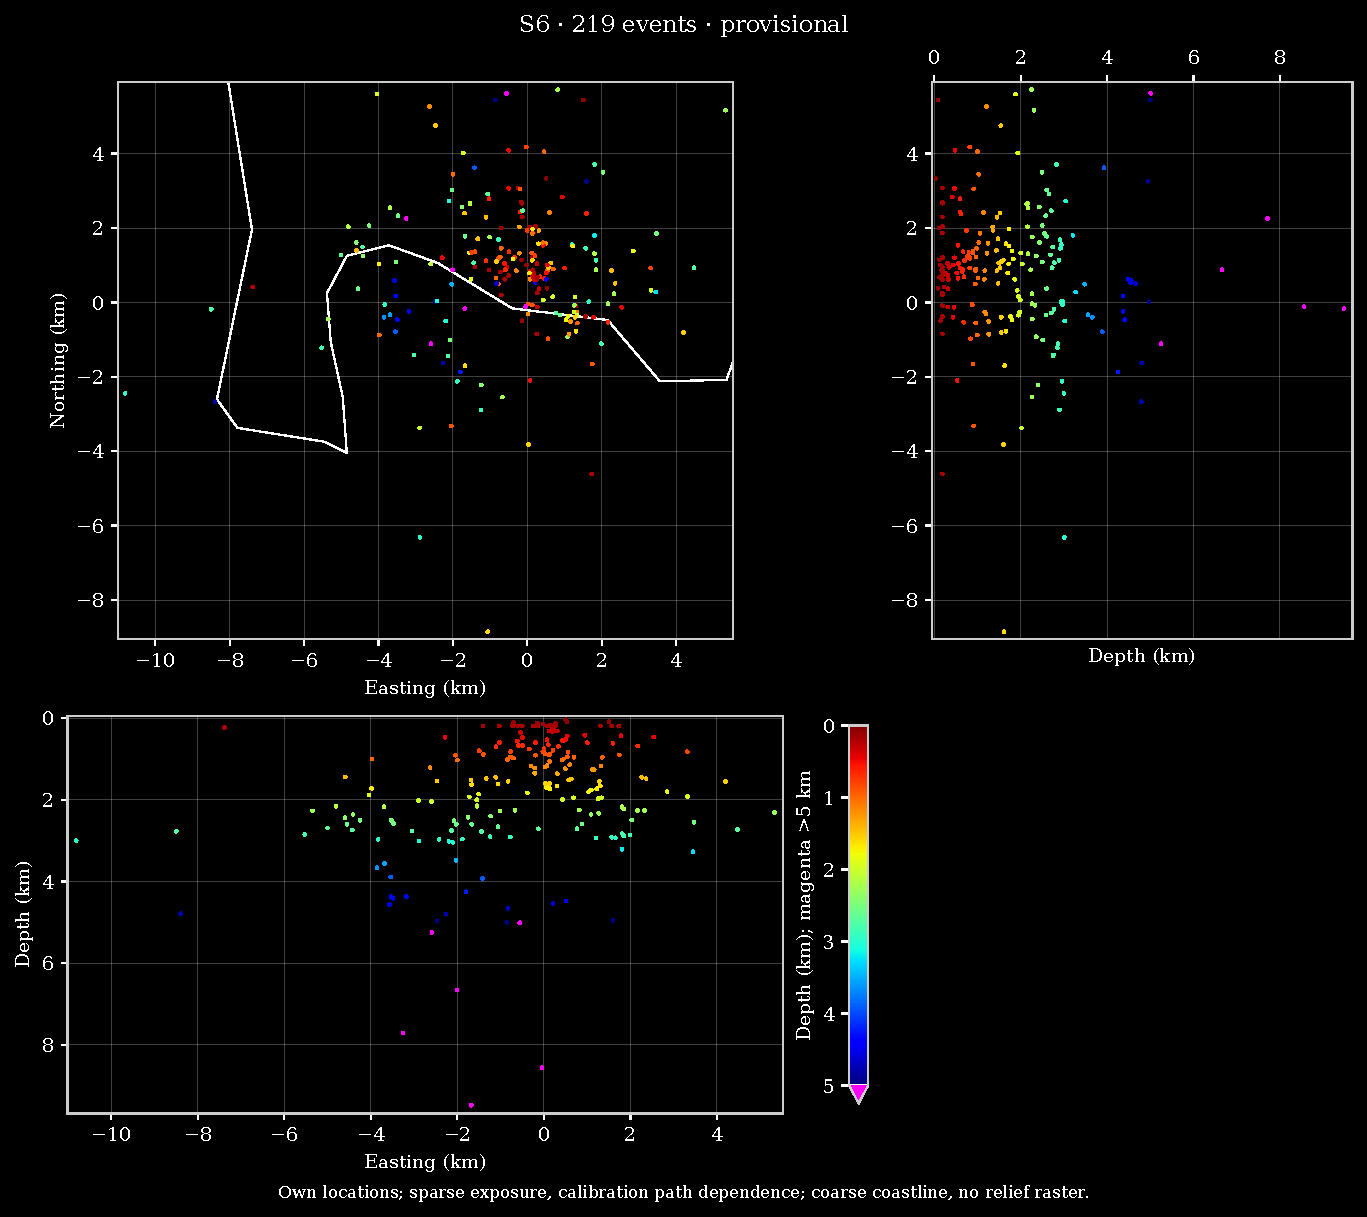
\includegraphics[width=.94\linewidth,height=0.310\textheight,keepaspectratio]{figures/figure_S6_extension.pdf}
\caption{Initial VELEST locations. 216 independently fitted VELEST events pass the numerical pick/RMS/gap filters. Physical layer ordering and the final small-update gate pass; stagnation, held-out prediction, regional and precision-path stability prevent acceptance. These are plotted as provisional results. Provisional independent observations and processing; sparse coverage, unreviewed phases, calibration path sensitivity. Not established fault geometry or exact reproduction. The additional extended-cohort view uses separately numbered, independently rerun results. Magnitudes and SVD uncertainties were not inherited by integer event ID.}
\label{publication:S6}
\end{figure}
